\documentclass[11pt,a4paper,spanish]{book}
\usepackage{estilo_unir-1}
\usepackage[nottoc]{tocbibind}
\usepackage{tikz}
\usetikzlibrary{arrows.meta,positioning}
\setlength{\headheight}{25.2842pt}
\hypersetup{
    colorlinks   = true,
    urlcolor     = blue,
    linkcolor    = black,
    citecolor   = red
}

%---------------------------
% título de la asignatura, trabajo y autor
%---------------------------
\subject{Protocolos cuánticos de seguridad y cifrado}
\title{Protocolos cuánticos de seguridad y cifrado. Posicionamiento, puntos fuertes y debilidades}
\author{Enrique Prada Vázquez, José Daniel Pérez Torres, Samuel Mascarell Martínez, Manuel Villa Arechaga, Urko Martín Marfull}
\profesor{Jenaro Gallego Gómez}
\date{18/05/2026}

\begin{document}
\renewcommand{\listfigurename}{Índice de figuras}
\renewcommand{\listtablename}{Índice de tablas}
\renewcommand{\contentsname}{Índice de contenidos}
\renewcommand{\figurename}{Figura}
\renewcommand{\tablename}{Tabla}

\maketitle
\frontmatter
\tableofcontents
\listoftables

\chapter{Resumen}


\vspace{0.5cm}
{\bf Palabras clave:} 
\chapter{Abstract}
This work analyzes the main discrete-variable quantum key distribution protocols, with the aim of systematically characterizing their foundations, strengths, and weaknesses. A structured literature review methodology was applied, using a uniform template for each protocol covering its physical principles, operational scheme, known vulnerabilities, and practical examples. The protocols studied are: BB84, B92, E91, six-state protocol, SARG04, decoy-state BB84, LM05, and MDI-QKD. Results reveal a clear evolution from simple prepare-and-measure schemes toward entanglement-based and measurement-device-independent proposals, each addressing specific limitations of its predecessors. It is concluded that no single protocol is universally optimal: the choice depends on the implementation scenario, available technological capabilities, and the assumed threat model, with decoy-state protocols and MDI-QKD representing the most mature solutions for real-world deployments.

\vspace{0.5cm}
{\bf Keywords:} quantum key distribution, quantum cryptography, discrete-variable protocols, quantum entanglement, decoy states, measurement-device independence

\mainmatter

\mainmatter

\chapter{Introducción}

\section{Motivación y justificación}

\section{Planteamiento del Trabajo}

\section{Estructura del Trabajo}

\chapter{Objetivos}

\section{Objetivo general}
Diferenciar las características más importantes, puntos fuertes y debilidades de los principales protocolos de intercambio de claves cuánticas de variable discreta, mediante un análisis comparativo y la ejemplificación práctica de sus fundamentos.

\section{Objetivos específicos}
\begin{itemize}
    \item Establecer un marco analítico uniforme y normalizado que permita evaluar de manera sistemática los fundamentos teóricos y operativos de los protocolos estudiados.
    \item Modelar el flujo operativo de cada protocolo mediante escenarios de aplicación originales y supuestos prácticos de diseño propio, fundamentados en la literatura científica actual.
    \item Evaluar el comportamiento de los esquemas de variable discreta frente a las vulnerabilidades físicas y amenazas críticas más relevantes, tales como los ataques de división del número de fotones, interceptación-reenvío y las limitaciones de los canales reales.
    \item Correlacionar de forma comparativa las propiedades, requisitos de infraestructura y niveles de seguridad de cada alternativa para determinar su viabilidad técnica en entornos de red.
\end{itemize}

\chapter{Enunciado del problema}

Se plantea desarrollar una descripción comparativa de los protocolos de intercambio de claves de variable discreta. Para ello se requiere seleccionar un marco común de análisis y aplicarlo a todos los protocolos. Dicho marco debe recoger las características principales, fundamentos, puntos fuertes, puntos débiles y una explicación práctica con ejemplos.

En este Trabajo se interpreta el problema como una comparación razonada de protocolos DV-QKD. No se pretende demostrar formalmente la seguridad composable de cada esquema, sino explicar sus mecanismos esenciales y su posicionamiento. Por ello se combinan referencias fundacionales con una lectura práctica orientada a la toma de decisiones: qué aporta cada protocolo, qué supuestos exige, qué ataques intenta mitigar y en qué contexto puede ser preferible.
\chapter{Desarrollo del Trabajo}

Este capítulo desarrolla el análisis central del Trabajo. En primer lugar, se presentan los conceptos básicos de la distribución cuántica de claves de variable discreta y el marco común empleado para comparar los protocolos. A continuación, se estudian de forma individual los principales protocolos seleccionados, manteniendo para todos ellos los mismos criterios: contexto y propósito, funcionamiento del protocolo, ventajas principales, limitaciones y riesgos, y ejemplo práctico.

\section{Conceptos básicos de distribución cuántica de claves de variable discreta}

Antes de comparar protocolos concretos, conviene fijar algunos conceptos básicos. Según \cite{gisin2002}, la distribución cuántica de claves, o QKD, no es un algoritmo de cifrado de mensajes, sino un mecanismo para que dos partes legítimas, normalmente llamadas Alicia y Bob, generen una clave secreta compartida. Como explican \cite{lo2014}, esa clave puede utilizarse después en un cifrado simétrico clásico; la función de QKD es, por tanto, resolver el problema de distribución de claves, no sustituir a todos los mecanismos de cifrado. La propuesta original de \cite{bennett1984} ya muestra que la seguridad del intercambio no se basa únicamente en la dificultad computacional de un problema matemático, sino en propiedades físicas de los sistemas cuánticos; en implementaciones reales, este razonamiento debe completarse con un modelo explícito de los dispositivos empleados \citep{scarani2009,lo2014}.

En los protocolos de variable discreta, la información se representa mediante cúbits. De acuerdo con \cite{nielsen2010}, un cúbit es un sistema cuántico de dos niveles que puede codificar los valores lógicos 0 y 1 mediante estados físicos concretos. En una implementación óptica, por ejemplo, esos estados pueden corresponder a polarizaciones, fases o intervalos temporales de pulsos luminosos \citep{gisin2002,scarani2009}. Por este motivo, a nivel abstracto resulta más riguroso hablar de cúbits, aunque en la práctica muchos sistemas los implementen mediante fotones o pulsos ópticos atenuados \citep{gisin2002,lo2014}.

Un protocolo DV-QKD combina normalmente dos canales. El canal cuántico transporta los cúbits o los sistemas físicos que los codifican, mientras que el canal clásico permite anunciar bases, descartar mediciones incompatibles, estimar errores, corregir discrepancias y aplicar amplificación de privacidad. Este canal clásico no necesita ser secreto, pero sí autenticado; de lo contrario, un atacante podría realizar un ataque de intermediario y hacerse pasar por una de las partes \citep{bennett1984, gisin2002,scarani2009,lo2014}.

Otro concepto central es el de base de preparación y medida. Como explican \cite{nielsen2010}, una base puede entenderse como un conjunto de estados distinguibles entre sí dentro de una misma medición. En la propuesta de \cite{bennett1984}, Alicia prepara cada cúbit en una de dos bases incompatibles, por ejemplo una base rectilínea o una base diagonal, y Bob elige la base con la que realiza la medición. Cuando ambos usan la misma base, el bit puede recuperarse con alta probabilidad en ausencia de ruido; cuando Bob mide en una base incompatible, el resultado pierde correlación con el estado preparado. Esta incompatibilidad introduce incertidumbre y perturbación ante mediciones no autorizadas, por lo que constituye uno de los mecanismos que permite detectar espionaje \citep{scarani2009}.

La seguridad básica se apoya en tres hechos. Primero, como demostraron \cite{wootters1982}, los estados cuánticos desconocidos no pueden copiarse perfectamente, principio conocido como teorema de no clonación. Segundo, medir en una base incompatible introduce perturbaciones estadísticas observables por Alicia y Bob \citep{bennett1984,nielsen2010}. Tercero, la información parcial que pudiera haber obtenido Eva puede reducirse mediante amplificación de privacidad, sacrificando parte de la clave reconciliada para producir una clave final más corta y más segura \citep{gisin2002,scarani2009}.

En una ejecución típica participan Alicia, que prepara estados, y Bob, que mide. Tras muchas rondas, ambos anuncian por el canal clásico parte de la información no secreta, por ejemplo las bases usadas \citep{bennett1984,gisin2002}. A partir de ahí calculan la tasa de error cuántico, o QBER, que mide la fracción de bits discrepantes entre Alicia y Bob en una muestra de la clave \citep{gisin2002,scarani2009}. Si el error supera un umbral, abortan porque el canal puede estar demasiado degradado o intervenido; si es aceptable, aplican reconciliación de información y amplificación de privacidad \citep{scarani2009,lo2014}.

La reconciliación de información es el procedimiento mediante el cual Alicia y Bob corrigen diferencias entre sus cadenas de bits sin revelar completamente la clave \citep{gisin2002,scarani2009}. Después, como señalan \cite{scarani2009}, la amplificación de privacidad transforma la clave corregida en una clave más corta sobre la que Eva tiene información despreciable dentro del modelo de seguridad considerado. Así, la clave final no procede de una única medición perfecta, sino de un procedimiento estadístico sobre muchas rondas.

También es importante distinguir entre seguridad teórica y seguridad de implementación. Un protocolo puede ser seguro en un modelo ideal, pero un sistema real incluye pérdidas, ruido, fuentes imperfectas, detectores no ideales y posibles canales laterales. Por ello, los protocolos modernos no solo especifican cómo preparar y medir cúbits, sino también qué supuestos se hacen sobre los dispositivos y qué contramedidas se necesitan frente a ataques prácticos \citep{scarani2009,lo2014}.
\input{capitulos/desarrollo/02_plantilla_analisis}
\section{Protocolo BB84}

\subsection{Contexto y propósito}
BB84 es el protocolo de referencia de la criptografía cuántica de variable discreta. Fue propuesto por \cite{bennett1984} y pertenece a la familia de preparación y medida \citep{gisin2002,scarani2009}. Su importancia no se limita a ser el primer protocolo QKD ampliamente reconocido: también sirve como modelo pedagógico y como base para variantes modernas, como BB84 con estados señuelo \citep{hwang2003,lo2005,wang2005}.

\subsection{Funcionamiento del protocolo}
El funcionamiento de BB84 puede entenderse como una secuencia de rondas independientes. En cada ronda, Alicia no envía directamente un bit clásico, sino un cúbit preparado de una forma concreta. Para ello elige dos elementos al azar: el valor del bit, que puede ser 0 o 1, y la base de codificación. En una descripción con polarización, la base rectilínea puede asociar el bit 0 a la polarización horizontal y el bit 1 a la vertical; la base diagonal puede asociar el bit 0 a 45 grados y el bit 1 a 135 grados \citep{bennett1984,gisin2002}.

Bob recibe cada cúbit sin saber qué base ha usado Alicia. Por tanto, también escoge al azar una base de medida. Si Bob elige la misma base que Alicia, obtiene el bit correcto con alta probabilidad en un canal ideal. Si elige la base equivocada, su resultado es esencialmente aleatorio y esa ronda no será útil para formar la clave \citep{bennett1984,scarani2009}.

Una vez transmitidos muchos cúbits, Alicia y Bob usan el canal clásico autenticado para comparar solo las bases empleadas, nunca los valores de los bits. Las rondas en las que ambos usaron bases distintas se descartan. Las rondas en las que usaron la misma base se conservan y forman una clave bruta, que todavía debe verificarse y depurarse \citep{gisin2002,scarani2009}.


\begin{figure}[h]
    \centering
    \begin{tikzpicture}[
        node distance=0.9cm and 1.3cm,
        paso/.style={draw, rounded corners, align=center, minimum width=3.6cm, minimum height=0.8cm},
        canal/.style={draw, rounded corners, align=center, minimum width=2.8cm, minimum height=0.8cm, fill=gray!10},
        flecha/.style={-{Latex[length=2mm]}, thick}
    ]
        \node[paso] (a1) {Alicia\\elige bit y base};
        \node[canal, right=of a1] (q) {canal cuántico\\cúbit};
        \node[paso, right=of q] (b1) {Bob\\elige base y mide};

        \node[paso, below=of a1] (a2) {Alicia anuncia\\su base};
        \node[canal, right=of a2] (c) {canal clásico\\autenticado};
        \node[paso, right=of c] (b2) {Bob anuncia\\su base};

        \node[paso, below=of c] (sift) {Cribado:\\se conservan solo\\bases coincidentes};
        \node[paso, below=of sift] (post) {Estimación de error,\\reconciliación y\\amplificación de privacidad};
        \node[paso, below=of post, fill=gray!10] (key) {Clave final\\compartida};

        \draw[flecha] (a1) -- (q);
        \draw[flecha] (q) -- (b1);
        \draw[flecha] (a1) -- (a2);
        \draw[flecha] (b1) -- (b2);
        \draw[flecha] (a2) -- (c);
        \draw[flecha] (b2) -- (c);
        \draw[flecha] (c) -- (sift);
        \draw[flecha] (sift) -- (post);
        \draw[flecha] (post) -- (key);
    \end{tikzpicture}
    \caption[Esquema operativo de BB84]{Diagrama de flujo simplificado del protocolo BB84. Fuente: elaboración propia.}
    \label{fig:bb84_flujo}
\end{figure}

La Figura~\ref{fig:bb84_flujo} resume esta lógica. El punto esencial es que Eva no conoce la base correcta durante la transmisión. Si intercepta un cúbit y lo mide, en muchas rondas elegirá una base incompatible. Al reenviar un nuevo cúbit a Bob, esa decisión introduce errores detectables en las rondas que Alicia y Bob conservan. Por ello, antes de aceptar la clave, ambos revelan públicamente una muestra de sus bits para estimar la tasa de error. Si el error es aceptable, aplican corrección de información y amplificación de privacidad; si es demasiado alto, abortan el protocolo \citep{bennett1984,scarani2009}.

\subsection{Ventajas principales}
\begin{itemize}
    \item Es conceptualmente simple y permite explicar de manera directa la relación entre medición cuántica y detección de espionaje.
    \item Cuenta con una gran tradición de análisis teórico y experimental.
    \item Puede implementarse con distintas codificaciones físicas, como polarización, fase o tiempo de llegada.
    \item Sirve como base de protocolos prácticos con estados señuelo, más adecuados para fuentes láser atenuadas.
\end{itemize}

\subsection{Limitaciones y riesgos}
\begin{itemize}
    \item La versión ideal presupone fuentes de cúbits físicos bien controlados y detectores perfectos, condiciones difíciles en sistemas reales.
    \item Las fuentes láser débiles pueden emitir pulsos multifotónicos, lo que abre la puerta a ataques de división de número de fotones.
    \item Los detectores reales pueden sufrir ataques laterales si el modelo de seguridad no representa fielmente el dispositivo.
    \item La mitad de las rondas se descartan en promedio por incompatibilidad de bases.
\end{itemize}

\subsection{Ejemplo práctico}
Se supone que Alicia desea generar una clave para cifrar los resultados preliminares de un laboratorio. Para ilustrar el procedimiento, se considera un caso reducido de seis rondas. Alicia elige una secuencia de bits y bases, prepara los cúbits correspondientes y los envía a Bob. Bob, sin conocer las bases de Alicia, mide cada cúbit con una base elegida al azar.

\begin{table}[h]
    \centering
    \small
    \begin{tabular}{c c c c c c}
        \hline\hline
        Ronda & Bit de Alicia & Base de Alicia & Base de Bob & ¿Coinciden? & Resultado \\
        \hline
        1 & 0 & Rectilínea & Rectilínea & Sí & Se conserva \\
        2 & 1 & Diagonal & Rectilínea & No & Se descarta \\
        3 & 1 & Rectilínea & Rectilínea & Sí & Se conserva \\
        4 & 0 & Diagonal & Diagonal & Sí & Se conserva \\
        5 & 1 & Diagonal & Rectilínea & No & Se descarta \\
        6 & 0 & Rectilínea & Diagonal & No & Se descarta \\
        \hline
    \end{tabular}
    \caption[Ejemplo de cribado en BB84]{Ejemplo simplificado de cribado de bases en BB84. Fuente: elaboración propia.}
    \label{tab:bb84_ejemplo}
\end{table}

En el caso de la Tabla~\ref{tab:bb84_ejemplo}, Alicia y Bob conservarían inicialmente las rondas 1, 3 y 4, porque en ellas ambos han usado la misma base. La clave bruta de Alicia sería, por tanto, 0, 1 y 0. En un canal ideal, Bob obtendría los mismos valores en esas rondas. Para comprobar si ha habido ruido o espionaje, podrían revelar públicamente una de las rondas conservadas, por ejemplo la ronda 3. Si ambos observan el mismo valor, continúan con las rondas restantes; si aparecen demasiadas discrepancias, abortan.

Si Eva hubiese interceptado los cúbits, tendría que medirlos sin conocer la base correcta. Cuando eligiera una base incompatible, modificaría el estado reenviado a Bob y aumentaría la probabilidad de error en las rondas conservadas. En una ejecución real no se usarían solo seis rondas, sino miles o millones, de modo que la estimación estadística del error fuera significativa. Este ejemplo es deliberadamente pequeño y solo pretende mostrar la lógica de preparación, medición, cribado y comprobación de errores.
\section{Protocolo B92}

El protocolo B92 representa un hito fundamental en la criptografía cuántica al demostrar que la seguridad no depende necesariamente de la cantidad de estados utilizados, sino de la propiedad de no ortogonalidad. En particular, este protocolo pone de manifiesto que incluso un conjunto mínimo de dos estados no ortogonales es suficiente para garantizar seguridad frente a un posible espía, debido a la imposibilidad de distinguirlos perfectamente sin introducir perturbaciones detectables (véase, por ejemplo, \cite{gisin2002}).

\subsection{Contexto y propósito}

El protocolo B92 \citep{bennett1992} es una variante simplificada de BB84 \citep{bennett1984} que emplea únicamente dos estados cuánticos no ortogonales \citep{schrodinger1926quantisierung} para codificar la información. Esta reducción disminuye la complejidad conceptual y experimental del sistema, manteniendo la seguridad basada en la imposibilidad de distinguir dichos estados sin introducir perturbaciones.

\subsection{Funcionamiento del protocolo}

El funcionamiento del protocolo B92 se articula en torno al uso de estados no ortogonales, lo que impide que un posible espía pueda obtener información sin alterar el sistema. A partir de este principio, el proceso se desarrolla de forma secuencial en varias fases:

\paragraph{1. Preparación y envío de estados}. Alice genera una secuencia aleatoria de bits clásicos. A continuación, 
codifica cada bit en un estado cuántico:

\begin{itemize}
    \item El bit 0 se codifica como el estado $|0\rangle$ (polarización horizontal).
    \item El bit 1 se codifica como el estado $|{+}\rangle$ (polarización diagonal).
\end{itemize}

Estos estados son no ortogonales, lo que significa que no pueden distinguirse con certeza absoluta mediante una única medición. Alice envía estos estados, uno a uno, a Bob a través de un canal cuántico.

\paragraph{2. Medición de los estados}. Para cada estado recibido, Bob selecciona aleatoriamente una de las dos bases de medida posibles:

\begin{itemize}
    \item La base $\mathcal{B}_0 = \{|0\rangle, |1\rangle\}$.
    \item La base $\mathcal{B}_+ = \{|{+}\rangle, |{-}\rangle\}$.
\end{itemize}

Debido a la no ortogonalidad de los estados enviados por Alicia, en muchos casos 
Bob no puede determinar con certeza qué estado fue enviado. Sin embargo, en 
determinadas situaciones obtiene un resultado concluyente:

\begin{itemize}
    \item Si detecta $|1\rangle$, sabe que Alicia no envió $|0\rangle$, por lo 
    que deduce que el bit era 1.
    \item Si detecta $|{-}\rangle$, sabe que Alicia no envió $|{+}\rangle$, por 
    lo que deduce que el bit era 0.
\end{itemize}

En el resto de los casos, el resultado es ambiguo y se descarta.

\paragraph{3. Filtrado y comparación}

Una vez que Bob ha realizado las mediciones, ambos participantes utilizan un canal clásico autenticado para coordinarse y extraer la información útil del proceso cuántico.  
  
En esta fase, Bob comunica a Alice exclusivamente las posiciones de los fotones para los cuales ha obtenido un resultado concluyente. Es importante destacar que Bob no revela el valor del bit medido, sino únicamente qué posiciones son válidas.  
  
A partir de esta información:  
  
\begin{itemize}  
    \item Alice identifica los bits que corresponden a esas posiciones. 
    \item Ambos descartan todos los eventos no concluyentes.  
\end{itemize}  
  
El resultado de este proceso es una secuencia común de bits denominada \textit{clave en bruto}.  
  
Posteriormente, Alice y Bob realizan una comparación parcial de esta clave y seleccionan aleatoriamente un subconjunto de bits y los comparan públicamente para estimar la tasa de error \textit{QBER} \citep{nielsen2010quantum}.  
  
\begin{itemize}  
    \item Si los valores coinciden en la mayoría de los casos, el canal se considera seguro.  
    \item Si aparece un número significativo de discrepancias, se concluye que ha habido interferencias o un posible ataque, y el protocolo se aborta.  
\end{itemize}  
  
Este procedimiento permite detectar la presencia de un espía, ya que cualquier medición no autorizada introduce perturbaciones en los estados cuánticos, lo que se refleja en un aumento del error en la clave compartida. Como se describe detalladamente en \cite{nielsen2010}, esta detección es posible porque las leyes de la mecánica cuántica impiden obtener información sobre el estado sin modificarlo inevitablemente.

\subsubsection{Codificación de estados}
En la fase inicial, Alice transforma la información binaria clásica en estados cuánticos mediante la preparación de estados con polarizaciones específicas. A diferencia de otros protocolos, el esquema B92 utiliza una base de estados no ortogonales para representar los valores lógicos, tal como se detalla en la Tabla~\ref{tab:codificacion_b92}, vinculando cada bit a un estado de polarización horizontal o diagonal.

\begin{table}[h!]
\label{tab:codificacion_b92}
\centering
\begin{tabular}{ccc}
\hline
\textbf{Bit} & \textbf{Estado} & \textbf{Polarizaci\'{o}n} \\
\hline
0 & $|0\rangle$ & Horizontal (0\textdegree) \\
1 & $|{+}\rangle$ & Diagonal (+45\textdegree) \\
\hline
\end{tabular}
\caption{Codificaci\'{o}n en B92. Fuente: elaboración propia}
\end{table}

\subsubsection{Medición de Bob}

Por su parte, Bob emplea un sistema de detección basado en bases de medida proyectivas diseñadas para identificar el estado ortogonal al que Alice podría haber enviado. Como se resume en la Tabla~\ref{tab:medicion_bob}, esta estrategia permite a Bob obtener un resultado concluyente solo cuando el fotón se detecta en la orientación opuesta al estado codificado, descartando cualquier medición ambigua derivada de la no ortogonalidad. Bob solo acepta resultados concluyentes (detección del estado ortogonal).

\begin{table}[h!]
\label{tab:medicion_bob}
\centering
\begin{tabular}{ccc}
\hline
\textbf{Base} & \textbf{Estados} & \textbf{Detecta} \\
\hline
$\mathcal{B}_0$ & $\{|{0}\rangle, |{1}\rangle\}$ & $\ket{+}$ \\
$\mathcal{B}_+$ & $\{|{+}\rangle, |{-}\rangle\}$ & $\ket{0}$ \\
\hline
\end{tabular}
\caption{Bases de medida. Fuente: elaboración propia.}
\end{table}

\subsubsection{Diagrama de flujo del protocolo}

Con el fin de facilitar la comprensión de la lógica secuencial que rige el protocolo B92, se presenta a continuación un diagrama de flujo  en el que se detallan las etapas críticas de la comunicación. En este esquema se visualiza cómo la seguridad radica en el filtrado de resultados no concluyentes y en la interacción necesaria entre el canal cuántico de envío y el canal clásico de validación.

\begin{figure}[h!]
\centering
\begin{tikzpicture}[node distance=3.2cm, every node/.style={draw, rectangle, rounded corners, align=center, font=\small, minimum height=1.2cm}]

% Nodos
\node (alice) {Alicia envía\\$\ket{0}$ o $\ket{+}$};
\node (bob) [right of=alice] {Bob mide en\\base aleatoria};
\node (decision) [right of=bob] {¿Resultado\\concluyente?};
\node (yes) [right of=decision, xshift=0.5cm] {Guardar bit y\\comunicar pos.};
\node (no) [above of=yes, node distance=1.5cm] {Descartar\\fotón};

% Flechas
\draw[->, thick] (alice) -- (bob);
\draw[->, thick] (bob) -- (decision);
\draw[->, thick] (decision) -- node[anchor=south] {Sí} (yes);
\draw[->, thick] (decision) |- node[anchor=west, yshift=0.6cm] {No} (no);

\end{tikzpicture}
\caption{Flujo operativo del protocolo B92. Fuente: elaboración propia.}
\label{fig:flujo_b92_horizontal}
\end{figure}

Como se observa en la Figura~\ref{fig:flujo_b92_horizontal}, el flujo resalta el carácter determinista de los bits aceptados por Bob tras la detección de estados ortogonales, reduciendo significativamente la probabilidad de compromiso de la clave compartida antes de las fases finales de post-procesamiento.

\subsection{Ventajas principales}

El protocolo B92 presenta una serie de ventajas que lo sitúan como una alternativa relevante dentro del panorama de los protocolos DV-QKD, ofreciendo un esquema simplificado que mantiene garantías de seguridad incondicional frente a ataques generales \citep{tamaki2003}, destacando principalmente por su extrema simplicidad al requerir únicamente dos estados cuánticos para su funcionamiento. Esta característica constituye su mayor fortaleza, ya que permite una implementación experimental mucho más sencilla que la del protocolo BB84, reduciendo significativamente la complejidad técnica y el diseño del hardware necesario. Asimismo, su seguridad se apoya en un fundamento teórico directo basado en la no ortogonalidad de los estados, permitiendo simplificar la arquitectura del sistema sin comprometer los principios esenciales de la mecánica cuántica que garantizan la confidencialidad en el intercambio de la clave.

%------------------------------------------------------

\subsection{Limitaciones y riesgos}
A pesar de su simplicidad, el protocolo B92 presenta limitaciones que condicionan su uso en entornos reales. Su baja eficiencia en la generación de clave, cercana al 25\% (véase Tabla~\ref{tab:comparativa_b92_bb84}), junto con una mayor sensibilidad al ruido del canal, lo sitúan en desventaja frente a alternativas más robustas, como BB84 con estados señuelo, especialmente en implementaciones de larga distancia o en canales con alta atenuación. En este contexto, \cite{wang2005} mostró que el uso de técnicas de estados señuelo permite reforzar la seguridad de los sistemas prácticos frente a los ataques de tipo \textit{Photon Number Splitting} (PNS), cuya base teórica y peligrosidad en fuentes no ideales fueron formalmente establecidas por \cite{brassard2000pns}. Esta vulnerabilidad es crítica en B92, ya que las imperfecciones en la fuente de los estados pueden permitir a un adversario obtener información de la clave sin introducir el nivel de ruido previsto por el protocolo original.

\begin{table}[h!]
\label{tab:comparativa_b92_bb84}
\centering
\begin{tabular}{ccc}
\hline
\textbf{Característica} & \textbf{B92} & \textbf{BB84} \\
\hline
Estados & 2 & 4 \\
Bases & Implícitas & 2 explícitas \\
Eficiencia & $\sim 25\%$ & $\sim 50\%$ \\
Complejidad & Baja & Media \\
Robustez al ruido & Menor & Mayor \\
Uso práctico & Limitado & Estándar \\
\hline
\end{tabular}
\caption{Comparación entre B92 y BB84. Fuente: elaboración propia.}
\end{table}

%------------------------------------------------------

\subsection{Ejemplo práctico}

A continuación se presenta una ejecución simplificada del protocolo B92 con el objetivo de ilustrar su funcionamiento real. En este ejemplo, Alice genera una secuencia de seis bits aleatorios y los codifica en los estados cuánticos correspondientes, mientras que Bob aplica sus bases de medida de forma aleatoria.


Como se observa en la Tabla~\ref{tab:ejemplo_b92}, únicamente las posiciones 1, 2, 5 y 6 producen resultados concluyentes, descartándose las posiciones 3 y 4 por resultar ambiguas. Esto refleja la eficiencia característica del protocolo, en torno al 66\%, donde solo una fracción de los cúbits enviados contribuye efectivamente a la clave en bruto.

\begin{table}[h!]
\centering
\caption{Ejecución del protocolo B92}
\label{tab:ejemplo_b92}
\begin{tabular}{cccccc}
\hline
\textbf{Pos.} & \textbf{Bit A} & \textbf{Estado} & \textbf{Base B} & \textbf{Resultado} & \textbf{Clave} \\
\hline
1 & 0 & $|0\rangle$ & $\mathcal{B}_+$ & $|{-}\rangle$ & 0 \\
2 & 1 & $|{+}\rangle$ & $\mathcal{B}_0$ & $|1\rangle$ & 1 \\
3 & 1 & $|{+}\rangle$ & $\mathcal{B}_+$ & $|{+}\rangle$ & -- \\
4 & 0 & $|0\rangle$ & $\mathcal{B}_0$ & $|0\rangle$ & -- \\
5 & 1 & $|{+}\rangle$ & $\mathcal{B}_0$ & $|1\rangle$ & 1 \\
6 & 0 & $|0\rangle$ & $\mathcal{B}_+$ & $|{-}\rangle$ & 0 \\
\hline
\end{tabular}
\end{table}

\[
\text{Clave final: } 0, 1, 1, 0
\]

\subsubsection{Presencia de un espía}

Si Eve intercepta los fotones, introduce errores en la clave. Al comparar una muestra, Alice y Bob detectan un aumento del QBER, lo que permite identificar el ataque y abortar la comunicación.

\begin{table}[h!]
\centering
\caption{Resumen técnico del protocolo B92}
\begin{tabular}{lp{8cm}}
\hline
\textbf{Parámetro} & \textbf{Descripción y Valor} \\
\hline
\textbf{Familia} & DV-QKD (Variable Discreta). \\
\textbf{Nº de estados} & 2 estados no ortogonales ($\ket{0}$ y $\ket{+}$). \\
\textbf{Nº de bases} & 2 bases de medida ($\mathcal{B}_0$ y $\mathcal{B}_+$). \\
\textbf{Eficiencia teórica} & 25\% (solo 1 de cada 4 fotones genera clave). \\
\textbf{Seguridad} & Basada en el principio de no clonación y discriminación de estados no ortogonales. \\
\textbf{Punto fuerte} & Extrema simplicidad en la preparación de estados. \\
\textbf{Punto débil} & Alta sensibilidad al ruido y baja tasa de generación de clave (\textit{key rate}). \\
\textbf{Estado actual} & Relevante teóricamente; uso práctico limitado frente a variantes de BB84 con estados señuelo. \\
\hline
\end{tabular}
\end{table}
\section{Protocolo E91}
 
\subsection{Contexto y propósito}
El protocolo E91 fue propuesto por \cite{ekert1991} y representa un cambio conceptual fundamental respecto a BB84 y B92. Mientras que los protocolos de preparación y medida basan su seguridad en la indistinguibilidad de estados cuánticos, E91 fundamenta la distribución de claves en el entrelazamiento cuántico y en la violación de las desigualdades de Bell \citep{ekert1991,gisin2002}. Esta distinción no es solo formal: en E91 la seguridad puede verificarse directamente a partir de correlaciones estadísticas medibles, sin necesidad de confiar en que la fuente de estados sea honesta, lo que lo conecta con el paradigma de la criptografía independiente del dispositivo \citep{scarani2009,acin2007}.
 
En E91, una fuente genera pares de cúbits entrelazados en el estado singlete de Bell y distribuye un cúbit de cada par a Alicia y otro a Bob. Si ningún adversario ha perturbado el estado, las mediciones de ambos sobre sus respectivos cúbits exhibirán correlaciones que violan la desigualdad CHSH, lo que certifica la presencia de entrelazamiento genuino y la ausencia de información filtrada a un espía \citep{ekert1991,clauser1969}.
 
\subsection{Funcionamiento del protocolo}
La fuente genera repetidamente el estado singlete $|\Psi^-\rangle = \frac{1}{\sqrt{2}}(|01\rangle - |10\rangle)$ y distribuye el primer cúbit a Alicia y el segundo a Bob \citep{ekert1991}. Alicia escoge aleatoriamente su dirección de medida entre tres ángulos; en la descripción original son $0$, $\pi/4$ y $\pi/2$ radianes. Bob escoge la suya entre otros tres ángulos: $\pi/4$, $\pi/2$ y $3\pi/4$ radianes \citep{ekert1991,gisin2002}.
 
Tras medir muchos pares, Alicia y Bob anuncian por el canal clásico autenticado los ángulos empleados en cada ronda, pero nunca los resultados obtenidos. Las rondas se dividen en dos grupos. En las rondas donde ambos eligieron bases coincidentes (los ángulos compartidos $\pi/4$ y $\pi/2$), los resultados están perfectamente anticorrelacionados para el estado singlete y se usan para formar la clave bruta. En las rondas con bases distintas, los resultados se emplean para estimar los coeficientes de la desigualdad CHSH \citep{ekert1991,clauser1969,scarani2009}.
 
\begin{figure}[h]
    \centering
    \begin{tikzpicture}[
        node distance=0.9cm and 1.2cm,
        paso/.style={draw, rounded corners, align=center, minimum width=3.4cm, minimum height=0.8cm},
        canal/.style={draw, rounded corners, align=center, minimum width=2.8cm, minimum height=0.8cm, fill=gray!10},
        flecha/.style={-{Latex[length=2mm]}, thick}
    ]
        \node[canal] (src) {Fuente\\par entrelazado $|\Psi^-\rangle$};
        \node[paso, left=1.4cm of src] (a1) {Alicia\\elige ángulo\\y mide};
        \node[paso, right=1.4cm of src] (b1) {Bob\\elige ángulo\\y mide};
 
        \node[canal, below=of src] (c) {canal clásico\\autenticado};
        \node[paso, left=1.4cm of c] (a2) {Alicia anuncia\\ángulos usados};
        \node[paso, right=1.4cm of c] (b2) {Bob anuncia\\ángulos usados};
 
        \node[paso, below=1.2cm of c, xshift=-2.2cm] (sift) {Rondas coincidentes:\\clave bruta};
        \node[paso, below=1.2cm of c, xshift=+2.2cm] (bell) {Rondas distintas:\\test CHSH};
 
        \node[paso, below=1.2cm of sift, xshift=+2.2cm] (post) {Reconciliación y\\amplificación de privacidad};
        \node[paso, below=of post, fill=gray!10] (key) {Clave final\\compartida};
 
        \draw[flecha] (src) -- (a1);
        \draw[flecha] (src) -- (b1);
        \draw[flecha] (a1) -- (a2);
        \draw[flecha] (b1) -- (b2);
        \draw[flecha] (a2) -- (c);
        \draw[flecha] (b2) -- (c);
        \draw[flecha] (c) -- (sift);
        \draw[flecha] (c) -- (bell);
        \draw[flecha] (sift) -- (post);
        \draw[flecha] (bell) -- (post);
        \draw[flecha] (post) -- (key);
    \end{tikzpicture}
    \caption[Esquema operativo de E91]{Diagrama de flujo simplificado del protocolo E91. Fuente: elaboración propia.}
    \label{fig:e91_flujo}
\end{figure}
 
La Figura~\ref{fig:e91_flujo} resume la estructura del protocolo. Si Eva ha interceptado o manipulado los cúbits, el entrelazamiento original se habrá degradado y las correlaciones medidas en las rondas de test no alcanzarán el valor esperado por la mecánica cuántica. En ese caso, la desigualdad CHSH deja de violarse, y Alicia y Bob detectan la anomalía estadística y abortan el protocolo \citep{ekert1991,scarani2009}. Si la violación se confirma, continúan con la clave bruta, aplican corrección de errores y amplificación de privacidad \citep{gisin2002}.
 
\subsection{Ventajas principales}
\begin{itemize}
    \item La seguridad se certifica a través de un test físico observable, la violación de la desigualdad CHSH, lo que elimina la necesidad de asumir que la fuente de estados es honesta o que los dispositivos se comportan como se anuncia \citep{ekert1991,acin2007}.
    \item La fuente de pares entrelazados puede encontrarse en un nodo intermedio no confiable, ya que cualquier manipulación por parte de ese nodo se reflejaría en las estadísticas de Bell \citep{gisin2002,scarani2009}.
    \item E91 constituye el precedente conceptual directo de los protocolos independientes del dispositivo, que representan el estándar más alto de seguridad demostrable en QKD \citep{acin2007}.
    \item Admite implementaciones con fotones entrelazados en polarización, tiempo o grado de libertad orbital, lo que ofrece flexibilidad en la elección de la plataforma física \citep{gisin2002}.
\end{itemize}
 
\subsection{Limitaciones y riesgos}
\begin{itemize}
    \item La generación y distribución eficiente de pares entrelazados es tecnológicamente más exigente que la simple preparación de estados de un fotón, lo que eleva el coste y la complejidad de la implementación experimental \citep{gisin2002}.
    \item La tasa de generación de clave es menor que en BB84, ya que solo las rondas con bases coincidentes contribuyen a la clave bruta y las rondas de test consumen una fracción adicional de los pares generados \citep{scarani2009}.
    \item Las pérdidas del canal afectan a los dos brazos de distribución de forma independiente, lo que puede reducir severamente la tasa de detecciones en coincidencia, especialmente a larga distancia \citep{gisin2002}.
    \item El test CHSH requiere acumular suficientes rondas para que la estimación estadística sea significativa; en presencia de ruido elevado o baja eficiencia de detección, puede ser difícil obtener una violación estadísticamente concluyente \citep{ekert1991,scarani2009}.
\end{itemize}
 
\subsection{Ejemplo práctico}
Se supone que Alicia y Bob desean establecer una clave usando una fuente de pares entrelazados situada en un nodo intermedio. Para ilustrar el procedimiento, se considera un caso reducido de seis rondas. En cada ronda la fuente emite un par en el estado $|\Psi^-\rangle$, Alicia elige uno de sus tres ángulos de medida y Bob elige uno de los suyos, de forma independiente y aleatoria. Los conjuntos de ángulos posibles son $\{0, \pi/4, \pi/2\}$ para Alicia y $\{\pi/4, \pi/2, 3\pi/4\}$ para Bob; los ángulos compartidos son $\pi/4$ y $\pi/2$.
 
\begin{table}[h]
    \centering
    \small
    \begin{tabular}{c c c c c}
        \hline\hline
        Ronda & Ángulo de Alicia & Ángulo de Bob & ¿Bases coinciden? & Uso de la ronda \\
        \hline
        1 & $0$       & $\pi/4$   & No  & Test CHSH \\
        2 & $\pi/4$   & $\pi/4$   & Sí  & Clave bruta \\
        3 & $\pi/2$   & $3\pi/4$  & No  & Test CHSH \\
        4 & $\pi/2$   & $\pi/2$   & Sí  & Clave bruta \\
        5 & $0$       & $3\pi/4$  & No  & Test CHSH \\
        6 & $\pi/4$   & $\pi/2$   & No  & Test CHSH \\
        \hline
    \end{tabular}
    \caption[Ejemplo de cribado en E91]{Ejemplo simplificado de clasificación de rondas en E91. Fuente: elaboración propia.}
    \label{tab:e91_ejemplo}
\end{table}
 
En el caso de la Tabla~\ref{tab:e91_ejemplo}, solo las rondas 2 y 4 tienen bases coincidentes y pasan a formar parte de la clave bruta. Para el estado singlete, si Alicia obtuvo el bit 0 en la ronda 2, Bob habrá obtenido el bit 1, y viceversa; uno de los dos puede invertir su bit para que ambos compartan la misma cadena. Las rondas 1, 3, 5 y 6, con bases distintas, se usan para calcular el parámetro $S$ de la desigualdad CHSH. En presencia de entrelazamiento puro, el valor esperado es $S = 2\sqrt{2} \approx 2{,}83$, que viola el límite clásico $S \leq 2$ \citep{clauser1969}. Si las rondas de test arrojan un valor de $S$ compatible con el límite clásico, Alicia y Bob concluyen que el estado ha sido perturbado y abortan el protocolo. Este ejemplo reducido tiene únicamente como propósito ilustrar la lógica de distribución de pares, clasificación de rondas y verificación de seguridad mediante el test de Bell que caracteriza al protocolo E91.

\section{Protocolo de seis estados}

Después de la propuesta de BB84 de \cite{bennett1984}, la distribución cuántica de claves por preparación y medida quedó establecida como una forma de aprovechar la incompatibilidad de bases para detectar posibles intervenciones externas. El protocolo de seis estados, propuesto por \cite{bruss1998}, puede leerse como una continuación natural de esa idea, pues mantiene la lógica de preparación, medición y cribado, pero añade una tercera base de codificación. Esta ampliación conecta con la noción de bases mutuamente no sesgadas introducida por \cite{schwinger1960} y permite estudiar de manera más simétrica la relación entre elección de bases, perturbación por medición y detección de espionaje.

\subsection{Contexto y propósito}

El protocolo de seis estados es una extensión directa de la idea de distribución cuántica de claves por preparación y medida introducida en BB84 \citep{bennett1984}. Su formulación específica fue propuesta para usar los seis autoestados de las tres matrices de \cite{pauli1927}, es decir, dos estados por cada una de las bases asociadas a $X$, $Y$ y $Z$ \citep{bruss1998}. La motivación central es aumentar la simetría del protocolo, pues en lugar de emplear dos bases mutuamente no sesgadas, como en BB84, Alicia y Bob usan tres bases mutuamente no sesgadas, concepto introducido en la teoría cuántica por \cite{schwinger1960}.

Esta mayor simetría puede visualizarse en la esfera de \cite{bloch1946}, que es una representación geométrica del estado de un sistema cuántico de dos niveles. En esa representación, las tres bases asociadas a $X$, $Y$ y $Z$ corresponden a tres ejes distintos; por ello, una medición no autorizada puede introducir perturbaciones detectables en más direcciones de análisis. Así, el protocolo de seis estados se estudia como una alternativa conceptualmente cercana a BB84, pero con una estimación de error más informativa frente a ataques individuales o incoherentes \citep{bruss1998,bechmann1999}.

\subsection{Funcionamiento del protocolo}

En cada ronda, Alicia elige aleatoriamente un bit clásico y una de tres bases de preparación. Si usa la base $Z$, puede codificar los bits en $\left|0\right\rangle$ y $\left|1\right\rangle$; si usa la base $X$, en $\left|+\right\rangle$ y $\left|-\right\rangle$; y si usa la base $Y$, en los dos autoestados de la matriz de Pauli $Y$ \citep{pauli1927,bruss1998}. Estas tres parejas de estados forman seis posibles señales cuánticas, de donde procede el nombre del protocolo \citep{bruss1998}.

Bob, sin conocer la elección de Alicia, selecciona también al azar una de las tres bases y mide el cúbit recibido. La regla operativa es la misma que en BB84: cuando ambos usan la misma base, el resultado de Bob coincide con el bit preparado por Alicia en un canal ideal; cuando usan bases distintas, el resultado no se conserva para la clave porque las bases mutuamente no sesgadas producen resultados uniformemente aleatorios entre sí \citep{schwinger1960,bennett1984}.

Después de muchas rondas, Alicia y Bob comunican públicamente las bases usadas mediante un canal clásico autenticado, pero no revelan los valores de todos los bits \citep{bennett1984}. Solo conservan las rondas en las que las bases coinciden; como hay tres bases equiprobables, la fracción ideal de rondas conservadas es aproximadamente un tercio \citep{bruss1998}. A partir de una muestra de esas rondas estiman la tasa de error cuántico, descartan la ejecución si el error es demasiado alto y, si continúa el protocolo, aplican reconciliación de información y amplificación de privacidad, técnicas introducidas en criptografía cuántica y clásica moderna por \cite{brassard1994}, y por \cite{bennett1995}, respectivamente.

\begin{figure}[h]
    \centering
    \begin{tikzpicture}[
        node distance=0.85cm and 0.95cm,
        paso/.style={draw, rounded corners, align=center, minimum width=3.1cm, minimum height=0.85cm},
        canal/.style={draw, rounded corners, align=center, minimum width=2.7cm, minimum height=0.85cm, fill=gray!10},
        proceso/.style={draw, rounded corners, align=center, minimum width=4.4cm, minimum height=0.85cm},
        flecha/.style={-{Latex[length=2mm]}, thick}
    ]
        \node[paso] (alice-prep) {Alicia\\elige bit y base\\$X$, $Y$ o $Z$};
        \node[canal, right=of alice-prep] (quantum-channel) {Canal cuántico\\uno de seis estados};
        \node[paso, right=of quantum-channel] (bob-measure) {Bob\\elige base y mide\\$X$, $Y$ o $Z$};

        \node[paso, below=of alice-prep] (alice-basis) {Alicia\\anuncia su base};
        \node[canal, right=of alice-basis] (classical-channel) {Canal clásico\\autenticado};
        \node[paso, right=of classical-channel, xshift=0.77cm] (bob-basis) {Bob\\anuncia su base};

        \node[proceso, below=of classical-channel] (sifting) {Cribado: se conservan solo\\las bases coincidentes};
        \node[proceso, below=of sifting] (postprocessing) {Estimación de error, reconciliación\\y amplificación de privacidad};
        \node[proceso, below=of postprocessing, fill=gray!10] (final-key) {Clave final compartida};

        \draw[flecha] (alice-prep) -- (quantum-channel);
        \draw[flecha] (quantum-channel) -- (bob-measure);
        \draw[flecha] (alice-prep) -- (alice-basis);
        \draw[flecha] (bob-measure) -- (bob-basis);
        \draw[flecha] (alice-basis) -- (classical-channel);
        \draw[flecha] (bob-basis) -- (classical-channel);
        \draw[flecha] (classical-channel) -- (sifting);
        \draw[flecha] (sifting) -- (postprocessing);
        \draw[flecha] (postprocessing) -- (final-key);
    \end{tikzpicture}
    \caption[Esquema operativo del protocolo de seis estados]{Diagrama de flujo simplificado del protocolo de seis estados. Fuente: elaboración propia.}
    \label{fig:seis_estados_flujo}
\end{figure}

La Figura~\ref{fig:seis_estados_flujo} muestra que el cambio esencial respecto a BB84 no está en la comunicación clásica posterior, sino en el alfabeto cuántico inicial. Al existir tres bases, Eva debe adivinar entre más opciones si intenta medir el cúbit durante la transmisión. Además, por el teorema de no clonación, no puede copiar un estado cuántico arbitrario desconocido para posponer la medición hasta que se anuncien las bases \citep{wootters1982}. La seguridad intuitiva del protocolo combina, por tanto, incompatibilidad de medidas, bases mutuamente no sesgadas y no clonación cuántica \citep{pauli1927,schwinger1960,wootters1982,bruss1998}.


\subsection{Ventajas principales}
\begin{itemize}
    \item Usa tres bases mutuamente no sesgadas, lo que proporciona una prueba de consistencia más simétrica que la de BB84 \citep{schwinger1960,bruss1998}.
    \item Permite estimar errores asociados a las tres componentes de \cite{pauli1927} del cúbit, no solo a dos familias de preparación \citep{bruss1998}.
    \item Es más sensible a ciertas estrategias de interceptación y reenvío, porque Eva debe escoger entre tres bases posibles \citep{bennett1984,bruss1998}.
    \item Mantiene una estructura operativa sencilla de preparación, medición, cribado y posprocesado, heredada de BB84 \citep{bennett1984}.
\end{itemize}

\subsection{Limitaciones y riesgos}
\begin{itemize}
    \item En la versión equiprobable, solo se conserva alrededor de un tercio de las rondas, porque Alicia y Bob deben coincidir en una de tres bases \citep{bruss1998}.
    \item Requiere preparar y medir también los estados de la base $Y$, lo que añade exigencias experimentales frente a implementaciones que solo usan dos bases \citep{pauli1927,bruss1998}.
    \item El modelo ideal presupone que cada ronda queda descrita por un único sistema de dos niveles preparado en una de las seis señales del protocolo; si esa hipótesis se relaja, el análisis de seguridad deja de coincidir con la formulación teórica original \citep{bennett1984,bruss1998}.
    \item La seguridad práctica depende de que los dispositivos reales representen fielmente el modelo teórico, especialmente en detectores y moduladores \citep{bruss1998,bechmann1999}.
\end{itemize}

\subsection{Ejemplo práctico}

Supóngase que Alicia quiere generar una clave breve para compartir un resultado preliminar con Bob. En una ejecución reducida de nueve rondas, Alicia elige bits y bases entre $X$, $Y$ y $Z$, prepara uno de los seis estados del protocolo y lo envía por el canal cuántico \citep{bruss1998}. Bob mide cada cúbit en una base elegida al azar. Tras la transmisión, ambos anuncian únicamente las bases y conservan solo las rondas coincidentes, siguiendo el procedimiento de cribado introducido en BB84 \citep{bennett1984}.

\begin{table}[h]
    \centering
    \scriptsize
    \begin{tabular}{c c c c c c c c}
        \hline\hline
        Ronda & Bit de Alicia & Base de Alicia & Estado & Base de B & Bit de Bob & ¿Coinciden? & Resultado \\
        \hline
        1 & 0 & $Z$ & $|0\rangle$ & $Z$ & 0 & Sí & Se conserva \\
        2 & 1 & $X$ & $|-\rangle$ & $Y$ & -- & No & Se descarta \\
        3 & 0 & $Y$ & $|y_+\rangle$ & $Y$ & 0 & Sí & Se conserva \\
        4 & 1 & $Z$ & $|1\rangle$ & $X$ & -- & No & Se descarta \\
        5 & 0 & $X$ & $|+\rangle$ & $X$ & 0 & Sí & Se conserva \\
        6 & 1 & $Y$ & $|y_-\rangle$ & $Z$ & -- & No & Se descarta \\
        7 & 1 & $X$ & $|-\rangle$ & $X$ & 1 & Sí & Se conserva \\
        8 & 0 & $Z$ & $|0\rangle$ & $Y$ & -- & No & Se descarta \\
        9 & 1 & $Y$ & $|y_-\rangle$ & $Y$ & 1 & Sí & Se conserva \\
        \hline
    \end{tabular}
    \caption[Ejemplo de cribado en el protocolo de seis estados]{Ejemplo simplificado de cribado en el protocolo de seis estados. Fuente: elaboración propia.}
    \label{tab:seis_estados_ejemplo}
\end{table}

En la Tabla~\ref{tab:seis_estados_ejemplo}, las rondas 1, 3, 5, 7 y 9 sobreviven al cribado porque las bases de Alicia y Bob coinciden; esta comparación pública de bases procede de BB84 y se aplica aquí al alfabeto de seis estados. En el modelo ideal de preparación y medida, cuando Alicia y Bob usan la misma base, Bob obtiene el mismo valor preparado por Alicia; por eso, en el ejemplo, la clave bruta queda formada por los bits $0,0,0,1,1$ \citep{bennett1984,bruss1998}. Las rondas restantes no aportan bits a la clave porque Bob midió en una base distinta; en bases mutuamente no sesgadas, esa medición no determina el bit preparado \citep{schwinger1960}. Para comprobar si hubo ruido o espionaje, Alicia y Bob podrían revelar una parte de las posiciones conservadas y calcular la tasa de error cuántico, tal como se plantea en BB84 \citep{bennett1984}; si el error observado es compatible con el umbral aceptado, continuarían con reconciliación de información y amplificación de privacidad \citep{brassard1994,bennett1995}.

Si Eva intercepta los estados sin conocer la base, debe escoger una medición entre $X$, $Y$ o $Z$, que son las tres bases del protocolo de seis estados \citep{bruss1998}. Cuando elige una base distinta de la usada por Alicia, la incompatibilidad de medidas asociada a los observables de \cite{pauli1927} y a las bases mutuamente no sesgadas altera estadísticamente el estado reenviado a Bob \citep{schwinger1960}. Al repetirse este efecto en muchas rondas, la muestra pública de comprobación revela un incremento de errores, mecanismo ya presente en BB84 y reforzado aquí por el uso simétrico de tres bases \citep{bennett1984,bruss1998}.

\section{Protocolo SARG04}

\subsection{Contexto y propósito}
Uno de las potenciales limitaciones del protocolo BB84 está relacionado con fuentes láser atenuadas y la posibilidad de ataques no reconocibles. El protocolo SAGR04  propuesto por \cite{sgar04}, que mantiene el mismo formato de nombres de protocolos (Scarani, Acín, Ribordy, Gisin, 2004) fue diseñado para reforzar esta vulnerabilidad del protocolo BB84, especialmente para el ataque conocido como PNS (photon-number-splittting), cuando se usan pulsos coherentes atenuados en lugar de un solo fotón.
\newline

El ataque PNS aprovecha que las fuentes de pulsos coherentes  usadas en QKD, pueden emitir ocasionalmente más de un fotón por pulso. Un atacante, Eva,  puede separar y retener uno o más fotones de esos pulsos múltiples sin introducir errores detectables en la señal enviada a Bob, y medirlos más tarde para obtener información sobre la clave secreta, lo que compromete la seguridad de protocolos como BB84.Es decir, Eva puede, aprovechando las perdidas del canal, ejecutar y modificar cierto número de fotones hasta el umbral de la estadística de número de fotones que observa Bob no sea distinguible de una fuente aleatoria con ciertas perdidas.  \cite{lutkenhaus2002} muestran que, en presencia de pérdidas altas, el PNS puede ser la estrategia dominante frente a otros ataques y reducen severamente la tasa segura si no se corrige el problema mediante técnicas como ''states decoy'' \citep{hwang2003} o protocolos alternativos como SGAR04.

\subsection{Funcionamiento del protocolo}

El protocolo SARG04  conserva la misma preparación física de los cuatro estados no ortogonales que BB84, pero modifica el anuncio clásico posterior para codificar la información mediante pares de estados en lugar de anunciar la base empleada.
\newline

Alicia envía pulsos en uno de los cuatro estados $\{|0\rangle,|1\rangle,|+\rangle,|-\rangle\}$ elegidos al azar y Bob mide en una de las dos bases (polarización rectilínea o diagonal) como en BB84. La diferencia clave de SARG04 es que, tras la transmisión, Alicia no anuncia la base sino un par de estados que contiene el estado realmente enviado, por ejemplo $(|0\rangle,|+\rangle)$. Dado ese par, el resultado de Bob puede ser «concluyente» (su medida es incompatible con exactamente uno de los dos estados del par) o «no concluyente» (su resultado es compatible con ambos), de modo que solo las posiciones concluyentes se conservan para la clave. Esta regla reduce la proporción de bits retenidos respecto a BB84 pero cambia la estadística disponible para un atacante: Eva, incluso si retiene un fotón de un pulso multifotón (ataque PNS), no puede saber a priori qué par anunciará Alicia y, por tanto, no siempre podrá convertir su fotón retenido en información útil sin riesgo de introducir discrepancias detectables en la fracción concluyente de eventos. En otras palabras, el anuncio de pares limita la cantidad de información que Eva puede obtener de un fotón retenido porque la probabilidad de que ese fotón sea tratado por Bob como concluyente depende del par anunciado y de la base de medida de Bob, y Eva no controla ni conoce esos anuncios al interceptar el pulso. Por eso SARG04 mejora la resistencia práctica frente al PNS en escenarios con fuentes láser atenuadas: compensa la ventaja estadística de Eva restringiendo las rondas útiles para Eva, a costa de una menor eficiencia de cribado.
\newline


En la práctica, SARG04 puede generar clave secreta a partir de pulsos de dos fotones en condiciones donde BB84 no lo haría, aunque con las contramedidas modernas (p. ej. decoy states) BB84 con estados decoy suele alcanzar tasas y distancias seguras superiores; por tanto, la ventaja de SARG04 es especialmente relevante en implementaciones sin decoy o con alta pérdida 
\newline


\begin{figure}[h]
    \centering
    \begin{tikzpicture}[
        node distance=0.9cm and 1.3cm,
        paso/.style={draw, rounded corners, align=center, minimum width=3.6cm, minimum height=0.8cm},
        destaque/.style={draw=black, line width=0.9pt, rounded corners, align=center, minimum width=3.6cm, minimum height=0.8cm, fill=yellow!20},
        canal/.style={draw, rounded corners, align=center, minimum width=2.8cm, minimum height=0.8cm, fill=gray!10},
        flecha/.style={-{Latex[length=2mm]}, thick}
    ]
        \node[paso] (a1) {Alicia\\elige bit y base};
        \node[canal, right=of a1] (q) {canal cuántico\\cúbit};
        \node[paso, right=of q] (b1) {Bob\\elige base y mide};

        \node[destaque, below=of a1] (a2) {Alicia anuncia\\par de estados};
        \node[canal, right=of a2] (c) {canal clásico\\autenticado};
        \node[destaque, right=of c] (b2) {Bob anuncia posi-\\ciones coincidentes};

         % bloque simplificado que agrupa lo común con BB84
         \node[paso, below=2.0cm of c, minimum width=6.4cm] (common) {Cribado y post‑procesado\\(estimación de error, reconciliación y\\amplificación de privacidad)\\ 
         Clave final compartida \\ \textit{(igual que BB84)}};

         % flechas
         \draw[flecha] (a1.east) -- (q.west);
         \draw[flecha] (q.east) -- (b1.west);
         \draw[flecha] (a1.south) -- (a2.north);
         \draw[flecha] (b1.south) -- (b2.north);
         \draw[flecha] (a2.east) -- (c.west);
         \draw[flecha] (b2.west) -- (c.east);
         \draw[flecha] (c.south) -- (common.north);


    \end{tikzpicture}
    \caption[Esquema operativo de SARG04 simplificado]{Diagrama de flujo simplificado del protocolo SARG04. Fuente: Elaboración propia}
    \label{fig:sarg04_flujo}
\end{figure}

La Figura~\ref{fig:sarg04_flujo} resume esta lógica. Toda la estructura es similar a la Figura~\ref{fig:bb84_flujo} excepto el punto donde Alicia en lugar de anunciar sus bases, ahora anuncia un par de estados, por ejemplo $(|0\rangle, |+\rangle )$, y al mismo tiempo Bob, en lugar de anunciar sus bases, ahora comunica solo las posiciones concluyentes con la información de Alicia. En el diagrama de flujo marcamos en color amarillo los cambios frente al protocolo BB84.

\subsection{Ventajas principales}
\begin{itemize}
    \item Mejora la seguridad práctica frente a fuentes de luz atenuadas, reduciendo significativamente la ventaja de una atacante utilizando técnicas de PNS.
    \item Especialmente en canales con alta perdida o donde no se pueden implementar otras técnicas como ''decoy states''.
    \item Conserva la misma preparación física de estados que BB84, por lo que es fácil de implementar reutilizando procesos, sistemas y canales existentes.
\end{itemize}

\subsection{Limitaciones y riesgos}
\begin{itemize}
    \item El número de eventos concluyentes es menor que en protocolo BB84, así que hay generar un mayor número de intentos, y por tanto es menos eficiente en el proceso de cribado de bits útiles.
    \item Sigue siendo vulnerable a otros problemas prácticos como en BB84 (fallos de dectectores, ataques laterales,..) si el modelo de seguridad no es realista.

\end{itemize}

\subsection{Ejemplo práctico}

Para ilustrar el procedimiento, se considera mismo caso reducido de seis rondas que en protocolo BB84.

\begin{table}[h]
\centering
\small
\begin{tabular}{c c c c c c c}
\hline\hline
Ronda & Bit de Alicia & Enviado & Anunciado & Base de Bob & Resultado Bob & ¿Concluyente? \\
\hline
1 & 0 & $|0\rangle$ & ${|0\rangle,|+\rangle}$ & Rectilínea & $|0\rangle$ & Sí \\
2 & 1 & $|1\rangle$ & ${|1\rangle,|-\rangle}$ & Rectilínea & $|0\rangle$ & No \\
3 & 1 & $|+\rangle$ & ${|+\rangle,|1\rangle}$ & Diagonal & $|+\rangle$ & Sí \\
4 & 0 & $|-\rangle$ & ${|-\rangle,|0\rangle}$ & Diagonal & $|+\rangle$ & No \\
5 & 1 & $|+\rangle$ & ${|+\rangle,|1\rangle}$ & Rectilínea & $|1\rangle$ & No \\
6 & 0 & $|0\rangle$ & ${|0\rangle,|+\rangle}$ & Diagonal & $|-\rangle$ & No \\
\hline
\end{tabular}
\caption[Ejemplo de cribado en SARG04]{Ejemplo simplificado de cribado en SARG04: solo se conservan las rondas con resultados concluyentes. Fuente: elaboración propia.}
\label{tab:sarg04_ejemplo}
\end{table}

En el caso de la Tabla~\ref{tab:sarg04_ejemplo} Alicia envía estados elegidos al azar entre $|0\rangle,|1\rangle,|+\rangle,|-\rangle$ y, tras la medición de Bob, anuncia para cada ronda un par de estados que contiene el estado realmente enviado. La columna “Resultado Bob” indica el resultado físico de su medida en la base que eligió, y la columna “¿Concluyente?” señala si ese resultado permite a Bob inferir sin ambigüedad (o con la certeza requerida por el protocolo) el bit de Alicia dado el par anunciado: solo las rondas concluyentes se conservan para la clave bruta. Por tanto, mientras en BB84 la decisión de conservar se basa en la coincidencia de bases (aprox. $50\%$ de las rondas) , en SARG04 la decisión se basa en la compatibilidad del resultado de Bob con el par anunciado por Alicia (aprox. $25\%$); esto reduce la fracción de rondas retenidas pero modifica la estadística que un atacante puede explotar y hace evidente la presencia de Eva. 
\newline

El procedimiento de comprobación de ruido y espionaje es análogo al descrito para BB84, con una diferencia en lo que se revela públicamente: tras conservar las rondas concluyentes, Alicia y Bob pueden comparar una de esas rondas al azar para estimar la tasa de error y distinguir ruido de posible intervención de Eva. Si Eva interceptó y retuvo fotones (ataque PNS), su información útil sobre la clave dependerá ahora no solo de haber acertado la base, sino también de que la ronda resultara concluyente después del anuncio del par—una circunstancia que ella no puede prever al momento de la interceptación. Por tanto, aunque en una ejecución real se usarán miles o millones de rondas para obtener estimaciones estadísticas fiables, la lógica básica es la misma: conservación de rondas concluyentes, revelación aleatoria de una fracción para estimar errores, y abortar si la tasa de discrepancias excede el umbral aceptable.
\section{BB84 con estados señuelo}

En esta sección se evalúa la variante de BB84 con estados señuelo (\emph{decoy states}), una modificación metodológica diseñada para cerrar la brecha entre el modelo teórico ideal y las limitaciones de la tecnología de emisión actual. A continuación, se examinan su contexto de desarrollo, las modificaciones en su flujo operativo respecto al protocolo original, un escenario práctico simulado, así como el balance de sus ventajas operativas y limitaciones tecnológicas remanentes.

\subsection{Contexto y propósito}
La motivación detrás de esta variante radica en la inexistencia práctica de fuentes de fotón único perfectas en entornos comerciales \citep{gisin2002, lo2014}. En los despliegues reales, Alice suele emplear fuentes de pulsos coherentes atenuados (WCP, \emph{Weak Coherent Pulses}) que emiten fotones siguiendo una distribución estadística de Poisson, lo que implica una probabilidad no nula de que algunos pulsos contengan múltiples fotones en el mismo estado cuántico \citep{lutkenhaus2002}. Esta debilidad permite al espía ejecutar el ataque de división de número de fotones (PNS, \emph{Photon-Number-Splitting}), mediante el cual intercepta los fotones excedentes sin alterar el estado del fotón remanente que llega a Bob, comprometiendo críticamente la seguridad del canal \citep{brassard2000pns}. 

La técnica de los estados señuelo, propuesta inicialmente por \cite{hwang2003} y formalizada matemáticamente por \cite{lo2005} y \cite{wang2005}, resuelve esta vulnerabilidad sin necesidad de modificar el hardware de detección. Su propósito es introducir pulsos de control con diferentes intensidades medias para estimar con precisión matemática las fluctuaciones estadísticas y las pérdidas del canal óptico, desacoplando la tasa de error observada de la seguridad de la clave final.

\subsection{Funcionamiento del protocolo}
El flujo operativo base comparte la estructura cuántica de preparación y medida del protocolo BB84 estándar \citep{bennett1984, scarani2009}, pero introduce una variación crítica en la etapa de emisión. En lugar de utilizar una intensidad de luz constante para todos los pulsos, Alice conmuta de forma aleatoria la potencia de su fuente láser entre varios niveles de intensidad media predefinidos: habitualmente denominados pulso de señal ($\mu$), pulso señuelo ($\nu$) y pulso de vacío ($0$). Bob realiza las mediciones de forma convencional utilizando sus bases aleatorias, sin conocer a qué grupo de intensidad pertenece cada pulso recibido.

Una vez finalizada la transmisión cuántica y ejecutado el cribado clásico de bases, Alice revela a través del canal clásico autenticado el nivel de intensidad asignado a cada ronda \citep{lo2005}. Dado que las pérdidas por atenuación en la fibra óptica afectan de igual manera a cualquier pulso luminoso independientemente de su intensidad, la tasa de detección o ganancia de Bob ($Y_n$) para cada fotón debe guardar una relación estadística proporcional y predecible. Si un atacante intenta extraer fotones mediante un ataque PNS, alterará de forma inevitable las estadísticas de ganancia y la tasa de error de fase (\emph{phase error rate}) de los estados señuelo respecto a los de señal \citep{wang2005}, permitiendo a Alice y Bob descubrir la intrusión mediante el cálculo de los límites inferiores de los pulsos monofotónicos durante el postprocesamiento de los datos.

\subsection{Ventajas principales}
El impacto de los estados señuelo en la criptografía cuántica práctica se fundamenta en su capacidad para aproximar el rendimiento de los sistemas reales al límite de seguridad teórico \citep{scarani2009, lo2014}. Sus principales fortalezas se resumen a continuación:
\begin{itemize}
    \item Inmunidad rigurosa frente al ataque PNS, garantizando la seguridad incondicional (\emph{information-theoretic security}) incluso al utilizar fuentes láser atenuadas convencionales \citep{lo2005, wang2005}.
    \item Incremento drástico tanto en la distancia máxima de transmisión segura como en la tasa de generación de clave final (\emph{key rate}) en canales con altas pérdidas ópticas \citep{scarani2004}.
    \item Viabilidad de implementación inmediata sobre la infraestructura de hardware existente de BB84, requiriendo únicamente modificaciones a nivel de lógica de control de software y la adición de moduladores de intensidad en el bloque de emisión.
\end{itemize}

\subsection{Limitaciones y riesgos}
A pesar de consolidar la seguridad de las fuentes ópticas, esta variante traslada la complejidad analítica hacia otros componentes del sistema, abriendo nuevos vectores de vulnerabilidad práctica \citep{scarani2009, lydersen2010}. Los desafíos y riesgos remanentes se detallan a continuación:
\begin{itemize}
    \item Incremento en la carga computacional del postprocesamiento debido a la necesidad de resolver ecuaciones de estimación estadística y análisis de clave finita (\emph{finite-key analysis}) más complejas para cada nivel de intensidad.
    \item Vulnerabilidad latente ante ataques de canal lateral (\emph{side-channel attacks}) dirigidos a las imperfecciones de los detectores de Bob o fallos de calibración en los moduladores de Alice, conocidos como ataques de hackeo por intensidad \citep{lydersen2010}.
    \item Dependencia extrema de la estabilidad temporal de la fuente láser; si las fluctuaciones reales de la intensidad media superan los márgenes estadísticos asumidos en el modelo matemático, el sistema puede generar estimaciones de seguridad erróneas o falsos positivos.
\end{itemize}

\subsection{Ejemplo práctico}
Para ilustrar el funcionamiento de este mecanismo frente a una amenaza, se considera un escenario donde Alice desea enviar una clave y utiliza tres niveles de intensidad: señal ($\mu$), señuelo ($\nu$) y vacío ($0$). Para este ejemplo simplificado de seis rondas, se asume que un atacante (Eva) monitoriza el canal e intenta aplicar el ataque PNS únicamente cuando detecta pulsos multifotónicos.

\begin{table}[h]
    \centering
    \small
    \begin{tabular}{c c c c c c}
        \hline\hline
        Ronda & Intensidad & Coincidencia & Estado del pulso & Acción de Eva & Resultado de Bob \\
        \hline
        1 & Señal ($\mu$) & Sí & Monofotónico & Bloquea & No detectado \\
        2 & Señuelo ($\nu$) & Sí & Monofotónico & Permite pasar & Detectado correctamente \\
        3 & Vacío ($0$) & Sí & Sin fotones & Ninguna & No detectado \\
        4 & Señal ($\mu$) & Sí & Multifotónico & Divide y mide fotón & Detectado correctamente \\
        5 & Señuelo ($\nu$) & No & Monofotónico & Permite pasar & Se descarta por base \\
        6 & Señal ($\mu$) & Sí & Monofotónico & Permite pasar & Detectado correctamente \\
        \hline
    \end{tabular}
    \caption[Ejemplo operativo con estados señuelo]{Simulación del comportamiento del canal con estados señuelo ante un intento de ataque. Fuente: elaboración propia.}
    \label{tab:decoy_ejemplo}
\end{table}

Tras el cribado de bases clásico expuesto en la Tabla~\ref{tab:decoy_ejemplo}, Alice revela qué rondas correspondían a estados señuelo y de vacío. Al analizar estadísticamente los datos, Alice y Bob calcularán cuántos pulsos señuelo ($\nu$) llegaron al detector en relación con los pulsos de señal ($\mu$). En un canal normal con pérdidas homogéneas, ambos tipos de pulsos se atenuarían de forma proporcional. Sin embargo, como Eva alteró selectivamente la transmisión al interceptar o bloquear fotones basándose en el número de fotones por pulso (afectando de forma desproporcionada a la intensidad $\mu$), las estadísticas de ganancia finales de los estados señuelo no coincidirán con las predicciones teóricas. Al constatar esta anomalía estadística en las rondas de control, los usuarios detectan la manipulación del canal y abortan la generación de la clave.

\section{Protocolo LM05}

El protocolo BB84 de \cite{bennett1984} y su simplificación B92 de \cite{bennett1992} se basan en una arquitectura de comunicación unidireccional: Alice prepara estados cuánticos y los envía a Bob a través de un canal. El protocolo LM05, propuesto por \cite{lucamarini2005}, rompe con esta estructura clásica al introducir el concepto de comunicación cuántica bidireccional (o de dos vías) determinista. En este esquema, el cúbit viaja de Bob a Alice y, tras ser manipulado por ella, regresa a Bob. A diferencia de protocolos bidireccionales previos como el \textit{Ping-Pong} \citep{bostrom2002}, la gran innovación de LM05 es que logra una transmisión segura e independiente sin necesidad de utilizar el entrelazamiento cuántico como recurso.

\subsection{Contexto y propósito}

El protocolo LM05 fue propuesto por \cite{lucamarini2005} para solventar una de las principales ineficiencias del protocolo BB84 \citep{bennett1984}: el descarte masivo de cúbits debido a la falta de coincidencia en las bases de medida. En LM05, como Bob es quien prepara el estado inicial y quien lo vuelve a medir al final del proceso, la base de preparación y la de medida siempre coinciden. Esto permite que, teóricamente, cada cúbit intercambiado en el modo de mensaje contribuya a la generación de la clave, aumentando drásticamente la eficiencia del protocolo.

La seguridad del sistema ya no descansa en la elección aleatoria de bases independientes por parte de dos usuarios, sino en la capacidad de Alice para alternar aleatoriamente entre un modo de codificación de mensaje y un modo de control \citep{lucamarini2005}. Cualquier espía (Eva) que intente interceptar el cúbit, ya sea en el viaje de ida (Bob a Alice) o en el de vuelta (Alice a Bob), introducirá perturbaciones en el estado cuántico que serán detectadas inevitablemente durante las rondas de control, garantizando así la confidencialidad de la clave mediante los principios fundamentales de la mecánica cuántica \citep{wootters1982}.

\subsection{Funcionamiento del protocolo}

El ciclo comienza cuando Bob prepara un cúbit en uno de los cuatro estados estándar mutuamente insesgados: $\{|0\rangle, |1\rangle, |+\rangle, |-\rangle\}$, y se lo envía a Alice a través del canal cuántico \citep{lucamarini2005}. Al recibirlo, Alice decide aleatoriamente operar en uno de dos modos posibles: modo de mensaje (CM) o modo de control (CC).

Si Alice elige el modo de mensaje, codifica su bit de información aplicando una operación unitaria al cúbit recibido: aplica la matriz identidad $I$ para codificar un $0$ lógico (dejando el estado intacto), o aplica una transformación $U$ (típicamente análoga a la matriz de Pauli $i\sigma_y$) para codificar un $1$ lógico, la cual invierte el estado independientemente de la base en la que Bob lo haya preparado. Tras operar, devuelve el cúbit a Bob. Bob mide el cúbit en la misma base en la que lo preparó; si el estado es el mismo, registra un $0$, y si ha cambiado al estado ortogonal, registra un $1$ \citep{lucamarini2005}.

Si Alice elige el modo de control, mide el cúbit recibido en una base aleatoria (rectilínea o diagonal) y prepara un nuevo cúbit en el estado medido para devolvérselo a Bob. Tras la transmisión cuántica, Alice anuncia públicamente en qué rondas actuó en modo de control y qué bases y resultados obtuvo, lo que permite a Bob contrastar si hubo alteraciones en el canal (presencia de Eva).

\begin{figure}[h]
    \centering
    \begin{tikzpicture}[
        node distance=1.2cm and 1.5cm,
        paso/.style={draw, rounded corners, align=center, minimum width=3.2cm, minimum height=0.8cm},
        canal/.style={draw, rounded corners, align=center, minimum width=2.8cm, minimum height=0.8cm, fill=gray!10},
        proceso/.style={draw, rounded corners, align=center, minimum width=4.4cm, minimum height=0.85cm},
        flecha/.style={-{Latex[length=2mm]}, thick}
    ]
        \node[paso] (b1) {Bob prepara cúbit\\en base aleatoria};
        \node[canal, below=of b1] (c1) {Canal cuántico (Ida)};
        \node[paso, right=1.5cm of c1] (a1) {Alice recibe y elige:\\Modo Mensaje o Control};
        
        \node[canal, below=of a1] (c2) {Canal cuántico (Vuelta)};
        \node[paso, left=1.5cm of c2] (b2) {Bob mide cúbit\\en la base original};

        \node[canal, below=1.2cm of b2, xshift=2.4cm] (c3) {Canal clásico\\autenticado};

        \node[proceso, below=1cm of c3, xshift=-2.4cm] (key) {Modo Mensaje:\\Clave bruta (determinista)};
        \node[proceso, below=1cm of c3, xshift=+2.4cm] (ctrl) {Modo Control:\\Estimación de error};

        \node[proceso, below=1.3cm of key, xshift=+2.4cm] (post) {Reconciliación y\\amplificación de privacidad};
        \node[proceso, below=of post, fill=gray!10] (final) {Clave final compartida};

        \draw[flecha] (b1) -- (c1);
        \draw[flecha] (c1) -- (a1);
        \draw[flecha] (a1) -- (c2);
        \draw[flecha] (c2) -- (b2);
        
        \draw[flecha] (a1) |- (c3);
        \draw[flecha] (b2) |- (c3);
        
        \draw[flecha] (c3) -- (key);
        \draw[flecha] (c3) -- (ctrl);
        \draw[flecha] (key) -- (post);
        \draw[flecha] (ctrl) -- (post);
        \draw[flecha] (post) -- (final);
    \end{tikzpicture}
    \caption[Esquema operativo de LM05]{Diagrama de flujo simplificado del protocolo bidireccional LM05. Fuente: elaboración propia.}
    \label{fig:lm05_flujo}
\end{figure}

La Figura~\ref{fig:lm05_flujo} muestra la arquitectura en "U" característica de LM05. A diferencia de E91, no hay fuente externa; Bob es simultáneamente emisor inicial y receptor final. El canal clásico posterior solo se utiliza para revelar qué rondas fueron de control, efectuar la estimación de la tasa de error cuántico (QBER) y realizar el posprocesado habitual \citep{lucamarini2005,scarani2009}.

\subsection{Ventajas principales}
\begin{itemize}
    \item Generación de clave determinista: no se descartan cúbits por incompatibilidad de bases entre emisor y receptor, lo que aumenta teóricamente la eficiencia frente a protocolos unidireccionales como BB84 \citep{lucamarini2005}.
    \item No requiere entrelazamiento cuántico, simplificando enormemente los requisitos tecnológicos del hardware en comparación con E91 o Ping-Pong \citep{ekert1991,bostrom2002}.
    \item Bob actúa como su propio emisor y medidor, lo que reduce la necesidad de alinear los sistemas de referencia entre los laboratorios de Alice y Bob con la misma precisión que en otros protocolos.
\end{itemize}

\subsection{Limitaciones y riesgos}
\begin{itemize}
    \item El cúbit debe viajar por el canal dos veces (ida y vuelta), lo que duplica el impacto de la atenuación y las pérdidas del medio de transmisión (como la fibra óptica), reduciendo la distancia máxima operativa.
    \item La arquitectura bidireccional introduce una vulnerabilidad específica a los ataques de tipo "caballo de Troya" (Trojan-horse attacks): Eva puede inyectar luz en el equipo de Alice para leer qué operación está aplicando, requiriendo el uso de aisladores y detectores de intensidad adicionales \citep{gisin2002}.
    \item Al ser un protocolo de preparación y medida, su seguridad depende de una calibración perfecta de los dispositivos, a diferencia de la seguridad independiente del dispositivo que ofrece E91 \citep{acin2007}.
\end{itemize}

\subsection{Ejemplo práctico}

Supóngase que Alice y Bob desean establecer una clave mediante el protocolo LM05 en una ejecución reducida de ocho rondas. Bob prepara aleatoriamente estados en las bases rectilínea ($Z$) o diagonal ($X$) y los envía. Alice decide aleatoriamente si operar en modo mensaje (para transmitir la clave aplicando $I$ o $U$) o en modo control (para medir y reenviar). Tras la comunicación cuántica, Alice anuncia los modos empleados por el canal clásico \citep{lucamarini2005}.

\begin{table}[h]
    \centering
    \small
    \begin{tabular}{c c c c c c c}
        \hline\hline
        Ronda & Bob prepara & Modo Alice & Operación/Medida Alice & Bob recibe & Bob deduce & Uso \\
        \hline
        1 & $|+\rangle$ & Mensaje (Bit 0) & Aplica identidad $I$ & $|+\rangle$ & Bit 0 & Clave \\
        2 & $|0\rangle$ & Mensaje (Bit 1) & Aplica inversor $U$ & $|1\rangle$ & Bit 1 & Clave \\
        3 & $|-\rangle$ & Control & Mide $|-\rangle$, envía $|-\rangle$ & $|-\rangle$ & (Verifica) & Test de error \\
        4 & $|1\rangle$ & Mensaje (Bit 0) & Aplica identidad $I$ & $|1\rangle$ & Bit 0 & Clave \\
        5 & $|0\rangle$ & Control & Mide $|+\rangle$, envía $|+\rangle$ & $|+\rangle$ \text{o} $|-\rangle$ & (Descartada) & Test de error \\
        6 & $|-\rangle$ & Mensaje (Bit 1) & Aplica inversor $U$ & $|+\rangle$ & Bit 1 & Clave \\
        7 & $|+\rangle$ & Mensaje (Bit 1) & Aplica inversor $U$ & $|-\rangle$ & Bit 1 & Clave \\
        8 & $|1\rangle$ & Control & Mide $|1\rangle$, envía $|1\rangle$ & $|1\rangle$ & (Verifica) & Test de error \\
        \hline
    \end{tabular}
    \caption[Ejemplo de clasificación de rondas en LM05]{Ejemplo simplificado de rondas en LM05. Fuente: elaboración propia.}
    \label{tab:lm05_ejemplo}
\end{table}

En la Tabla~\ref{tab:lm05_ejemplo}, las rondas 1, 2, 4, 6 y 7 corresponden al modo de mensaje. Como Bob conoce el estado inicial, la simple comparación con el estado final le permite deducir con un 100\% de certeza si Alice aplicó $I$ (bit 0) o $U$ (bit 1), conformando directamente la clave bruta \citep{lucamarini2005}. Las rondas 3, 5 y 8 son rondas de control. En la ronda 5, Alice midió en la base equivocada respecto a la de Bob, por lo que el estado se colapsó y Bob obtendrá un resultado aleatorio; estas rondas cruzadas se descartan durante el posprocesado. Sin embargo, en las rondas de control donde las bases de Alice y Bob coinciden (rondas 3 y 8), los resultados deben ser idénticos. Si Eva hubiera interceptado el cúbit en el viaje de ida o de vuelta, habría modificado el estado de estas rondas de control introduciendo una tasa de error (QBER) anómala. Si dicho error supera el umbral de seguridad, Bob y Alice abortan el protocolo por considerar el canal comprometido.

\section{Protocolo MDI-QKD}
 
\subsection{Contexto y propósito}
El protocolo de distribución de clave cuántica independiente del detector (MDI-QKD, del inglés \emph{Measurement-Device-Independent Quantum Key Distribution}) fue propuesto por \cite{lo2012} como solución directa a una clase de ataques que habían comprometido implementaciones reales de QKD. Los protocolos anteriores, como BB84 o B92, asumen que los detectores de fotones se comportan exactamente según el modelo teórico. En la práctica, sin embargo, los detectores presentan imperfecciones explotables: los ataques de cegado del detector, demostrados experimentalmente por \cite{lydersen2010}, permiten a un adversario controlar las mediciones de Bob sin introducir errores estadísticos detectables, rompiendo la seguridad práctica de esos sistemas.
 
MDI-QKD elimina completamente esta vulnerabilidad al trasladar la medición a un nodo intermedio no confiable, denominado Charlie \citep{lo2012,braunstein2012}. Alicia y Bob preparan y envían estados cuánticos, pero ninguno de los dos realiza mediciones sobre los fotones del otro. Charlie, que puede ser un adversario o un equipo defectuoso, realiza una medición de Bell y anuncia el resultado. La clave se deduce a partir de ese anuncio sin que la seguridad dependa de la honestidad ni de la calibración de Charlie \citep{lo2012,curty2014}.
 
\subsection{Funcionamiento del protocolo}
En cada ronda, Alicia y Bob preparan de forma independiente un cúbit cada uno, eligiendo al azar un bit y una base de codificación, igual que en BB84 \citep{lo2012,gisin2002}. Ambos envían sus cúbits a Charlie a través de sus respectivos canales cuánticos. Charlie realiza una medición de Bell conjunta sobre los dos fotones recibidos e intenta proyectarlos sobre uno de los cuatro estados de Bell. Anuncia públicamente cuál de los cuatro resultados ha obtenido, o si la medición ha fallado \citep{lo2012,braunstein2012}.
 
Alicia y Bob usan el canal clásico autenticado para comparar las bases empleadas en cada ronda. Las rondas en las que ambos usaron bases distintas se descartan. En las rondas con bases coincidentes, el resultado anunciado por Charlie permite a Bob deducir, a partir de su propio bit y del anuncio, cuál fue el bit de Alicia, salvo posiblemente una inversión de bit predecible \citep{lo2012,curty2014}. La clave bruta resultante se somete a estimación de error, reconciliación de información y amplificación de privacidad de la misma forma que en BB84 \citep{lo2012,scarani2009}.
 
\begin{figure}[h]
    \centering
    \begin{tikzpicture}[
        node distance=0.9cm and 1.2cm,
        paso/.style={draw, rounded corners, align=center, minimum width=3.2cm, minimum height=0.8cm},
        charlie/.style={draw, rounded corners, align=center, minimum width=3.2cm, minimum height=0.8cm, fill=gray!20},
        canal/.style={draw, rounded corners, align=center, minimum width=2.6cm, minimum height=0.8cm, fill=gray!10},
        flecha/.style={-{Latex[length=2mm]}, thick}
    ]
        \node[paso] (a1) {Alicia\\elige bit y base\\prepara cúbit};
        \node[charlie, right=1.3cm of a1] (ch) {Charlie\\(no confiable)\\medición de Bell};
        \node[paso, right=1.3cm of ch] (b1) {Bob\\elige bit y base\\prepara cúbit};
 
        \node[canal, below=of ch] (anuncio) {Charlie anuncia\\resultado de Bell};
 
        \node[paso, below=of anuncio] (sift) {Alicia y Bob\\comparan bases\\(canal clásico)};
 
        \node[paso, below=of sift] (post) {Estimación de error,\\reconciliación y\\amplificación de privacidad};
        \node[paso, below=of post, fill=gray!10] (key) {Clave final\\compartida};
 
        \draw[flecha] (a1) -- (ch) node[midway, above, font=\small] {cúbit};
        \draw[flecha] (b1) -- (ch) node[midway, above, font=\small] {cúbit};
        \draw[flecha] (ch) -- (anuncio);
        \draw[flecha] (anuncio) -- (sift);
        \draw[flecha] (sift) -- (post);
        \draw[flecha] (post) -- (key);
    \end{tikzpicture}
    \caption[Esquema operativo de MDI-QKD]{Diagrama de flujo simplificado del protocolo MDI-QKD. Fuente: elaboración propia.}
    \label{fig:mdiqkd_flujo}
\end{figure}
 
La Figura~\ref{fig:mdiqkd_flujo} ilustra la arquitectura del protocolo. La propiedad central es que Charlie no tiene acceso a los bits individuales de Alicia ni de Bob: su anuncio solo revela una relación entre los dos cúbits, que Alicia y Bob pueden explotar para correlacionar sus claves brutas sin exponer sus valores individuales \citep{lo2012,braunstein2012}. Si Charlie intenta manipular la medición, o si un adversario controla completamente los detectores de Charlie, el efecto se manifiesta como un aumento en la tasa de error observable en las rondas de test, que Alicia y Bob detectan antes de aceptar la clave \citep{lo2012,curty2014}.
 
\subsection{Ventajas principales}
\begin{itemize}
    \item Elimina por completo la necesidad de confiar en los detectores: toda vulnerabilidad asociada al lado de medición, incluidos los ataques de cegado del detector, queda excluida del modelo de amenaza \citep{lo2012,lydersen2010}.
    \item El nodo de medición de Charlie puede ser operado por un tercero no confiable o incluso por un adversario, lo que permite arquitecturas de red donde los nodos intermedios no necesitan ser seguros \citep{lo2012,braunstein2012}.
    \item Es compatible con fuentes láser atenuadas y la técnica de estados señuelo, lo que permite implementaciones prácticas sin necesidad de fuentes de un único fotón \citep{lo2012,curty2014}.
    \item Proporciona una base para redes QKD estrella, donde múltiples usuarios comparten un nodo central de medición sin que ese nodo tenga acceso a ninguna clave \citep{curty2014}.
\end{itemize}
 
\subsection{Limitaciones y riesgos}
\begin{itemize}
    \item La tasa de generación de clave es significativamente menor que en BB84, principalmente porque la probabilidad de que Charlie obtenga una detección en coincidencia disminuye con las pérdidas de los dos canales simultáneamente, lo que penaliza especialmente las distancias largas \citep{lo2012,curty2014}.
    \item La implementación experimental requiere que los fotones emitidos por Alicia y Bob sean indistinguibles en todos sus grados de libertad en el momento de llegar a Charlie, lo que impone requisitos estrictos de sincronización y control espectral \citep{lo2012,gisin2002}.
    \item Aunque MDI-QKD elimina los ataques al lado del detector, no cubre vulnerabilidades del lado de la preparación, como las imperfecciones en la modulación de estados o los ataques de canal lateral sobre las fuentes de Alicia y Bob \citep{scarani2009,curty2014}.
    \item La necesidad de sincronización precisa entre las dos fuentes y el nodo de Charlie añade complejidad operativa y puede reducir la estabilidad del sistema en entornos de despliegue real \citep{lo2012}.
\end{itemize}
 
\subsection{Ejemplo práctico}
Se supone que Alicia y Bob desean establecer una clave utilizando como nodo de medición un equipo de Charlie cuya fiabilidad no puede garantizarse. Para ilustrar el procedimiento, se considera un caso reducido de seis rondas. En cada ronda, Alicia y Bob preparan independientemente un cúbit usando la misma lógica de elección de bit y base que en BB84, y los envían simultáneamente a Charlie. Charlie realiza la medición de Bell e informa del resultado.
 
\begin{table}[h]
    \centering
    \small
    \begin{tabular}{c c c c c c}
        \hline\hline
        Ronda & Base de Alicia & Base de Bob & Resultado de Charlie & ¿Bases coinciden? & ¿Se conserva? \\
        \hline
        1 & Rectilínea & Rectilínea & $|\Phi^+\rangle$ & Sí  & Sí \\
        2 & Diagonal   & Rectilínea & $|\Psi^-\rangle$ & No  & No \\
        3 & Rectilínea & Rectilínea & Fallo            & Sí  & No \\
        4 & Diagonal   & Diagonal   & $|\Phi^-\rangle$ & Sí  & Sí \\
        5 & Rectilínea & Diagonal   & $|\Psi^+\rangle$ & No  & No \\
        6 & Diagonal   & Diagonal   & $|\Phi^+\rangle$ & Sí  & Sí \\
        \hline
    \end{tabular}
    \caption[Ejemplo de cribado en MDI-QKD]{Ejemplo simplificado de cribado en MDI-QKD. Fuente: elaboración propia.}
    \label{tab:mdiqkd_ejemplo}
\end{table}
 
En el caso de la Tabla~\ref{tab:mdiqkd_ejemplo}, se conservan las rondas 1, 4 y 6, que son aquellas en las que Alicia y Bob usaron la misma base y Charlie obtuvo una detección en coincidencia. La ronda 3 se descarta a pesar de que las bases coinciden, porque Charlie no logró una detección válida. A partir del resultado de Bell anunciado por Charlie en cada ronda conservada, Bob puede aplicar o no una corrección de bit sobre su valor para sincronizar su clave bruta con la de Alicia, según la correspondencia definida por el protocolo.
 
Para verificar la seguridad, Alicia y Bob revelan públicamente los valores de una muestra de las rondas conservadas y calculan la tasa de error. Si Charlie hubiese manipulado las mediciones, los estados reenviados o los anuncios, la tasa de error observada en la muestra sería anormalmente alta, lo que conduciría a abortar el protocolo. En una implementación real se usarían miles de rondas y la técnica de estados señuelo para estimar con precisión los parámetros del canal. Este ejemplo reducido tiene únicamente como propósito ilustrar la lógica de preparación simultánea, medición de Bell delegada en un nodo no confiable y cribado por coincidencia de bases que caracteriza al protocolo MDI-QKD.

\chapter{Conclusiones y líneas de trabajo futuro}

A lo largo del presente trabajo se ha desarrollado un análisis sistemático de diferentes metodologías de DV-QKD, contrastando sus fundamentos teóricos con las limitaciones físicas impuestas por los componentes de hardware comerciales. A continuación, se presentan las conclusiones globales derivadas de esta investigación, seguidas de una propuesta estructurada con las líneas de trabajo que definen la vanguardia de esta disciplina.

\section{Conclusiones}

La primera y más relevante conclusión de este estudio es que la seguridad teórica o incondicional de los sistemas cuánticos, basada en leyes de la física como el teorema de no clonación \citep{wootters1982}, se ve comprometida de forma crítica al trasladar los esquemas teóricos a entornos de implementación reales. La imperfección de las fuentes ópticas comerciales, dominadas por la emisión multi-fotónica estocástica de los pulsos coherentes atenuados, introduce vectores de vulnerabilidad severos, siendo el ataque de división del número de fotones la amenaza más destructiva en canales con altas pérdidas \citep{brassard2000pns, lutkenhaus2002}.

Frente a este escenario, la evaluación comparativa realizada en este Trabajo muestra que no existe un diseño único óptimo, sino que la selección de la arquitectura de red depende de un compromiso (\emph{trade-off}) de ingeniería entre la eficiencia del cribado clásico, la tolerancia a la atenuación del canal y la complejidad del hardware óptico utilizado:
\begin{itemize}
    \item Las arquitecturas basadas en \textbf{codificación estándar con intensidad constante} destacan por su simplicidad algorítmica y una alta eficiencia de cribado teórica del 50\%, pero su incapacidad intrínseca para segregar los pulsos monofotónicos de los multifotónicos limita drásticamente su distancia segura en redes reales, volviéndolas ineficaces ante tasas de pérdidas elevadas.
    \item Los esquemas basados en la \textbf{modulación dinámica de la intensidad media} de la fuente representan la solución más robusta y comercialmente viable para neutralizar los ataques de división de fotones. Al alterar de forma probabilística la potencia del láser, permiten calcular con rigor matemático cotas inferiores de ganancia monofotónica. Aunque incrementa la carga computacional en el postprocesamiento estadístico (\emph{finite-key analysis}), esta variante estira la distancia operativa de la fibra óptica a rangos metropolitanos avanzados con óptimas tasas de generación de clave (\emph{key rates}).
    \item Las variantes basadas en la \textbf{reconfiguración del anuncio clásico por conjuntos de estados} ofrecen una alternativa metodológica sumamente ingeniosa al modificar la etapa de postprocesamiento clásico para codificar la información en pares de estados en lugar de revelar las bases. Su gran ventaja es que aprovecha de manera segura los componentes multifotónicos sin requerir modificaciones en la potencia de emisión del hardware emisor. No obstante, su penalización en la eficiencia de cribado (reducida al 25\%) y su menor rendimiento en distancia frente a los métodos de modulación de intensidad las configuran como soluciones de nicho, ideales para enlaces de corta distancia con alta atenuación donde no se disponga de moduladores ópticos rápidos.
\end{itemize}

Finalmente, se concluye que los ataques de canal lateral (\emph{side-channel attacks}), tales como el cegado de detectores de avalancha mediante inyección de luz clásica \citep{lydersen2010}, constituyen el verdadero cuello de botella para la seguridad práctica de las redes de comunicaciones cuánticas contemporáneas. Esto demuestra que la validación de un sistema criptográfico cuántico no puede limitarse a la elegancia de sus demostraciones matemáticas, sino que requiere auditorías rigurosas de calibración y modelos de seguridad adaptados al comportamiento físico del hardware real.


\begin{thebibliography}{99}
\bibitem[Bennett (1992)]{Bennett1992} Bennett, C. H. (1992). Quantum cryptography using any two nonorthogonal states. \textit{Physical Review Letters}, {\bf 68}(21):3121--3124. doi: 10.1103/PhysRevLett.68.3121.
\bibitem[Bennett y Brassard (1984)]{BB84} Bennett, C.H. y Brassard, G. (1984).
Quantum cryptography: Public key distribution and coin tossing \emph{Proceedings of the IEEE International Conference on Computers, Systems and Signal Processing}, Bangalore, India, 175--179.
\bibitem[Ekert (1991)] {Ekert1991} Ekert, A. K. (1991).  Quantum cryptography based on Bell's theorem.  \textit{Physical Review Letters}, {\bf 67}(6):661--663.
\bibitem[Gidney y Ekerå (2021)]{Gidney2021} Gidney, C. y Eker\aa, M. (2021).
How to factor 2048 bit RSA integers in 8 hours using 20 million noisy qubits.
\textit{Quantum}, 5, 433. \href{https://doi.org/10.22331/q-2021-04-15-433}{10.22331/q-2021-04-15-433}.
\bibitem[Hwang (2003)]{hwang2003} Hwang, W.-Y. (2003) Quantum key distribution with high loss: Toward global secure communication, \textit{Physical Review Letters, vol. 91} , 57901. \href{https://arxiv.org/abs/quant-ph/0211153}{doi:10.1103/PhysRevLett.91.057901}. 
\bibitem[Lütkenhaus y Jahma (2002)]{lutkenhaus2002} Lütkenhaus, N. y Jahma, M. (2002). Quantum key distribution with realistic states: Photon‑number statistics in the photon‑number splitting attack, \textit{New Journal of Physics, vol. 4}, 44. \href{https://arxiv.org/pdf/quant-ph/0112147} {doi:10.1088/1367-2630/4/1/344} 
\bibitem[Scarani et al. (2004)]{Scarani2004} Scarani, V., Acín, A., Ribordy, G., y Gisin, N. (2004). Quantum cryptography protocols robust against photon number splitting attacks for weak laser pulse implementations. \textit{Physical Review Letters}, {\bf 92}(5):057901. doi: 10.1103/PhysRevLett.92.057901.
\bibitem[Shor y Preskill (2000)]{shor2000}
Shor, P.W. y Preskill, J. (2000). Simple proof of security of the BB84 quantum key distribution protocol, \textit{Physical Review Letters} {\bf 85}, 441.
{doi:10.1103/PhysRevLett.85.441.

\end{thebibliography}

\end{document}
